\documentclass{beamer}
\usepackage{graphicx}
\usepackage{xcolor}
\usetheme{Madrid}
%%% Colors
\definecolor{ForestGreen}{RGB}{34,139,34}
\usecolortheme[named=ForestGreen]{structure}

\usepackage{amsthm}
\title[Minority Move-Ins and Home Appreciation]{"Blockbusting" in the 21st Century?: Minority Move-ins and Neighborhood Home Value Appreciation}
\author{Emerson Schryver}
\begin{document}
\begin{frame}
    \maketitle
\end{frame}
\begin{frame}
\frametitle{Background}
\begin{itemize}
    \item Housing discrimination: long-running problem in US
    \item Common historical tactics: racial deed covenants, redlining, white flight, and blockbusting (Rothstein, 2017).
    \item Long-term effects:
    Deed covenants → Improved relative neighborhood quality (Sood, Ehrman-Solberg, 2024).
Redlining → Higher localized poverty (Appel, Nickerson, 2016).
Majority-Black neighborhoods → Lower quality of opportunity (Chetty et al., 2014).

    \item Modern discrimination persists:
    Lending disparities (Quillian, Lee, Honoré, 2020).
    Racial steering in real estate (Glenn, 2018).
    
\end{itemize}
\end{frame}
%%%%%%%%%%%%%%%%%%%%%%%%%%%%
\begin{frame}
\frametitle{Introduction}
\begin{itemize}
    \item Investigates whether minority move-ins suppress home-value appreciation, a key claim behind 1950s blockbusting.
    \item Uses loan data (Fannie Mae \& Freddie Mac), ACS data for normalization, and Zillow ZHVI for home prices.
    \item Methodology:
    Selects majority-white zip codes with minority move-ins (2009-2010).
    Tracks change in minority move-in share (2012-2013) as treatment.
    Analyzes home price appreciation over six years (until 2019).    
    \item Findings: The relationship between minority move-in share and home-value appreciation is unclear—while the treatment group shows lower appreciation, variation is extremely high.
\end{itemize}
\end{frame}
%%%%%%%%%%%%%%%%%%%%%%%%%%%%
\begin{frame}
\frametitle{Methodology}
\begin{itemize}
    \item Description of methods used
    \item Data collection techniques
    \item Analysis processes
\end{itemize}
\end{frame}
%%%%%%%%%%%%%%%%%%%%%%%%%%%%
\begin{frame}
\frametitle{Data}
    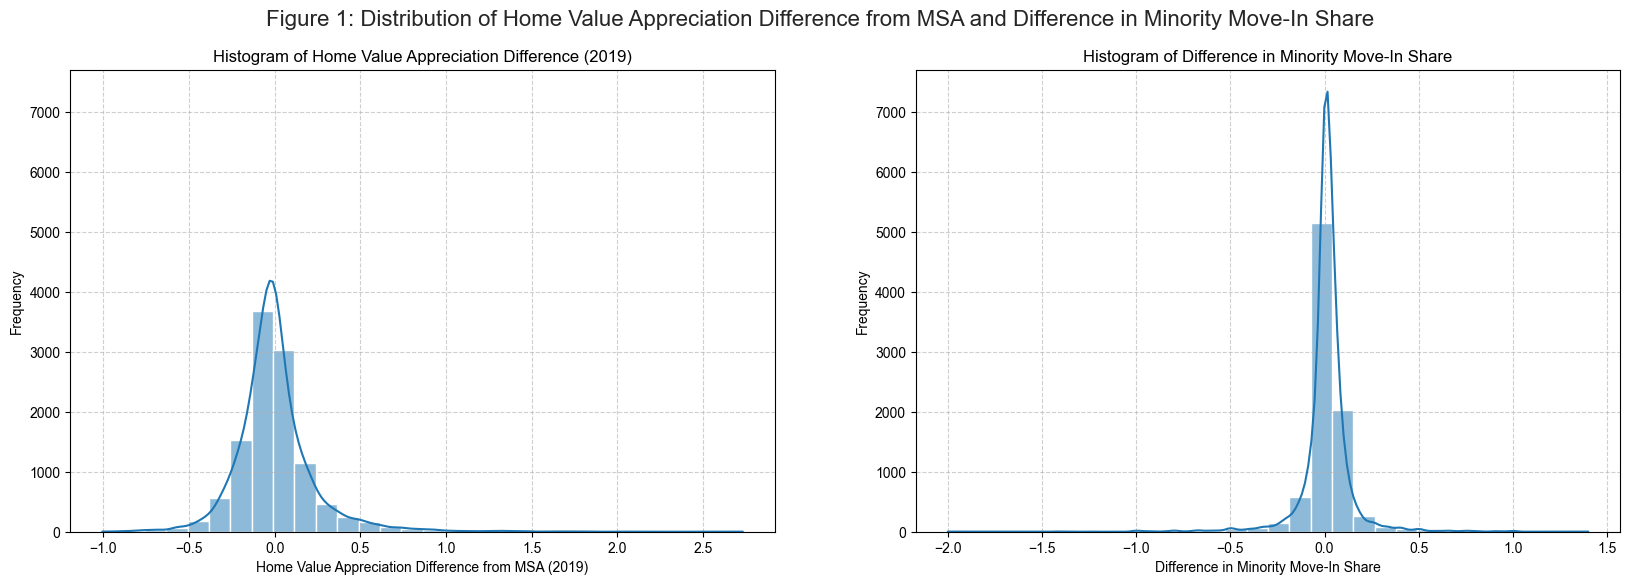
\includegraphics[width=\textwidth]{project_files/project_40_0.png}
\end{frame}
%%%%%%%%%%%%%%%%%%%%%%%%%%%%
\begin{frame}
\frametitle{Results}
\begin{itemize}
    \item Relatively inconclusive
    \item Some indication of suppression of home values but not significant
\end{itemize}
\end{frame}
%%%%%%%%%%%%%%%%%%%%%%%%%%%%
\begin{frame}
    \frametitle{Results}
    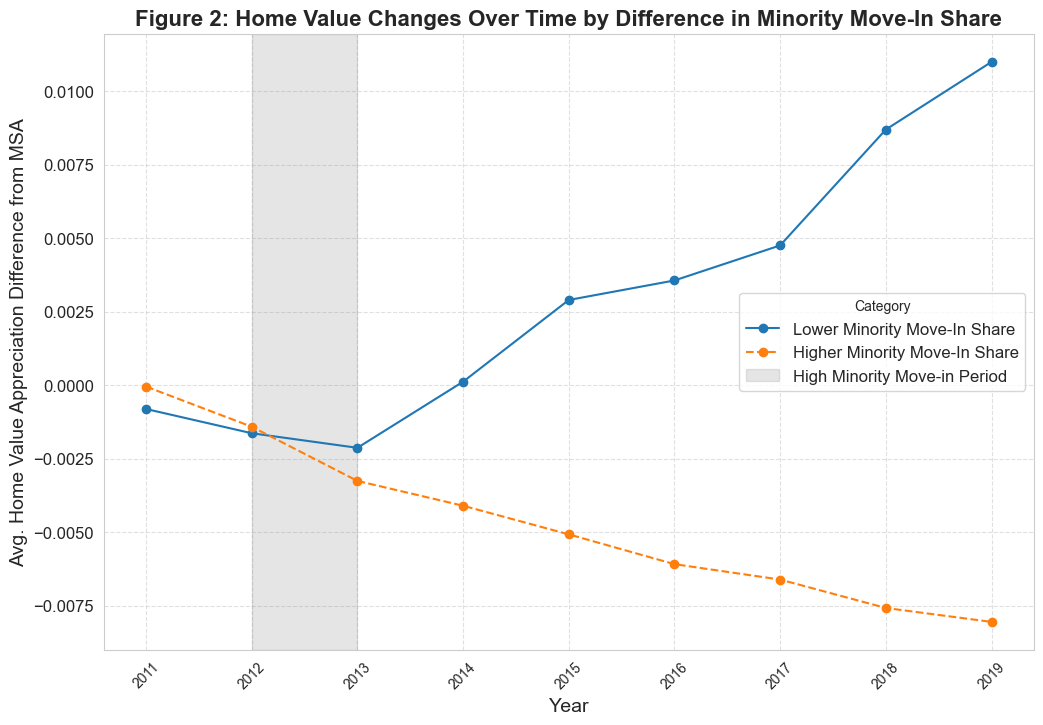
\includegraphics[width=\textwidth]{project_files/project_43_1.png}
\end{frame}
%%%%%%%%%%%%%%%%%%%%%%%%%%%%
\begin{frame}
    \frametitle{Results}
    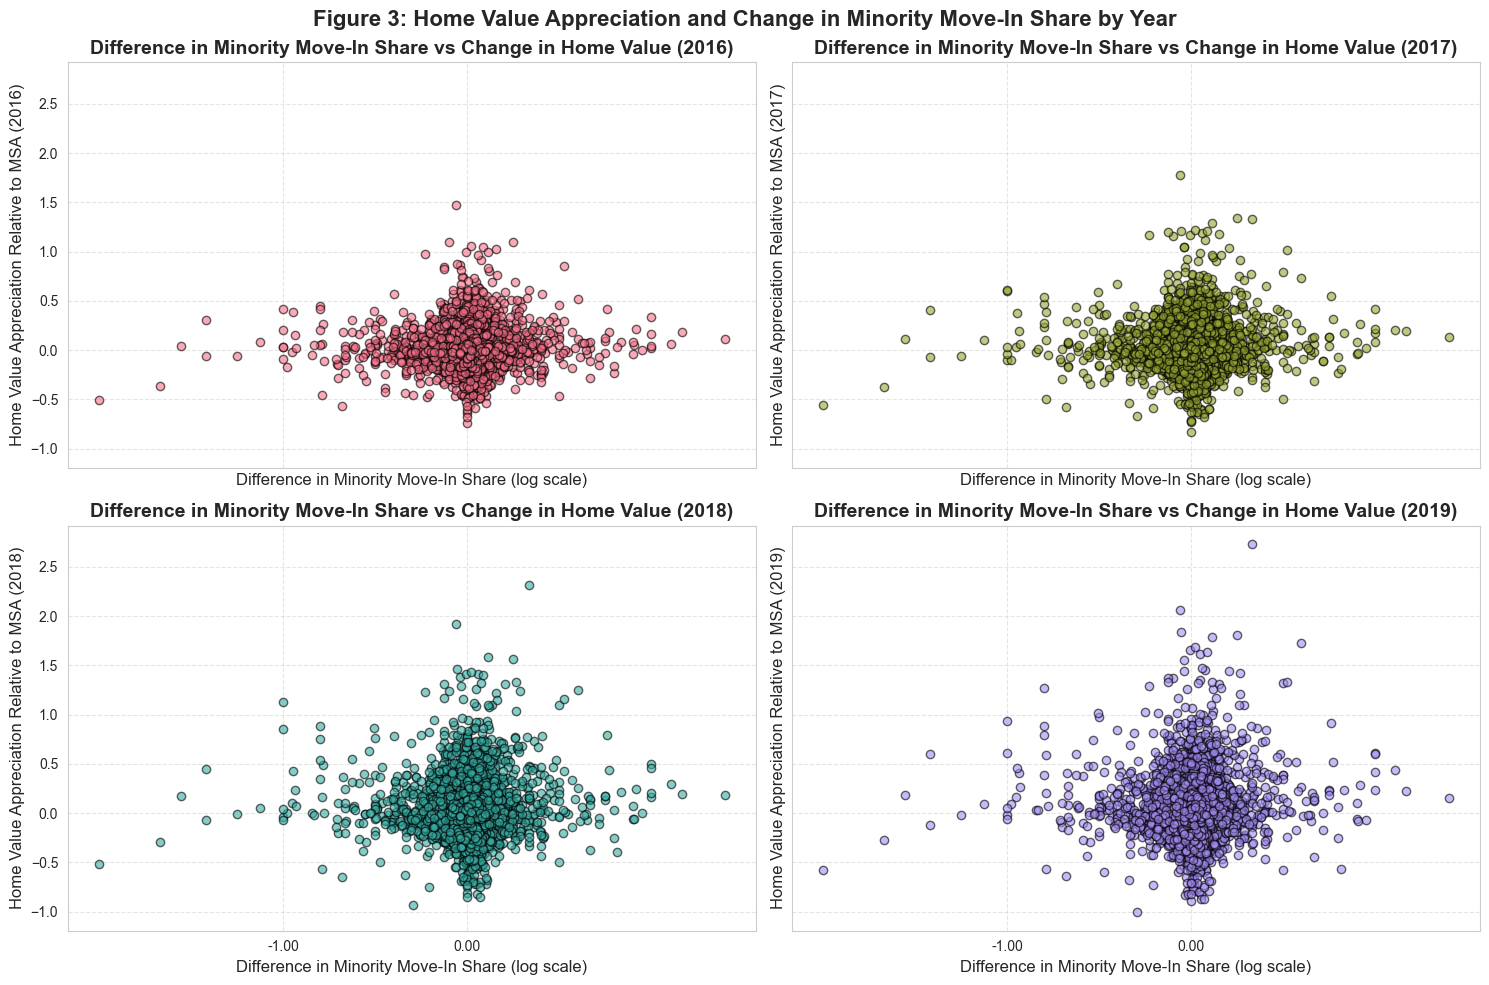
\includegraphics[width=\textwidth]{project_files/project_46_0.png}
\end{frame}
%%%%%%%%%%%%%%%%%%%%%%%%%%%%
\begin{frame}
    \frametitle{Results}
    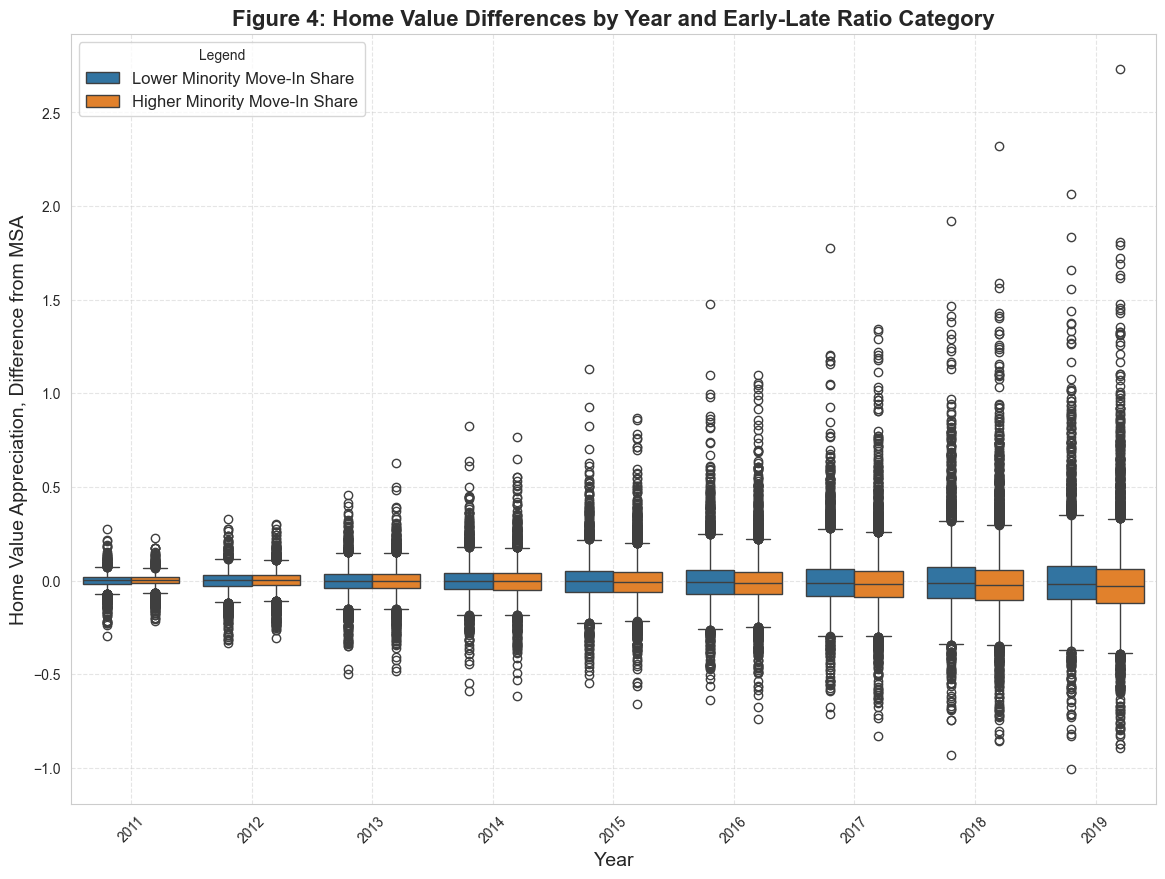
\includegraphics[width=\textwidth]{project_files/project_49_1.png}
\end{frame}
%%%%%%%%%%%%%%%%%%%%%%%%%%%%
\begin{frame}
\frametitle{Conclusion}
\begin{itemize}
    \item Summary of findings
    \item Limitations of study
    \item Future research
\end{itemize}
\end{frame}
\end{document}